% --
% thailand fotobuch

% document style
\documentclass{book}

% complex image tool
\usepackage{tikz}

% commands like left=of ...
\usetikzlibrary{positioning}

% arrow styles
\usetikzlibrary{arrows.meta}

% for layers
\usetikzlibrary{backgrounds, fit}

% animations?
\usetikzlibrary {animations}

% for coordinates
\usetikzlibrary{calc}

% fading and patterns
\usetikzlibrary{fadings, patterns}

% shadows
\usetikzlibrary{shadows}
\usetikzlibrary{shadows.blur}

% shapes?
\usetikzlibrary{shapes.symbols}

% remove page numbers
\pagestyle{empty}


% --
% tikz settings

\tikzset{help lines/.style={color=blue!60!orange, thick}}
\tikzset{rectStyle/.style={rectangle, draw=blue!50!green!50!black, fill=blue!50!green!25!white, thick, inner sep=0pt, minimum size=1cm}}
\tikzset{circStyle/.style={circle, draw=blue!80!green!50!black, fill=blue!70!green!25!white, thick, inner sep=0pt, minimum size=1cm}}
\tikzset{pre/.style={<-,shorten <=1pt,>={Stealth[round]},semithick}, post/.style={->,shorten >=1pt,>={Stealth[round]},semithick}}


% --
% document

\begin{document}

% line
\tikz{\draw (0, 0) -- (1, 1);}
% circle
\tikz{\fill[orange] (0, 0) circle (1);}
% triangle
\tikz{\draw (0, 0) -- (1, 0) -- (1, 1) -- cycle;}
% house of nikolaus
\tikz{\draw[thick, rounded corners=8pt] (0, 0) -- (0, 1) -- (0.5, 1.5) -- (1, 1) -- (1, 0) -- (0, 1) -- (1, 1) -- (0, 0) -- (1, 0);}
% circle stuff
\tikz{\draw (0, 0) .. controls (1, 1) and (2, 1) .. (2, 0)}
\tikz{\draw (0, 0) .. controls (0, 0.555) and (0.555, 1) .. (1, 1) .. controls (1.555, 1) and (2, 0.555) .. (2, 0);}
\tikz{\draw (0, 0) circle (1);}
% grid
\tikz{\draw (0, 0) rectangle (1, 2)}
\tikz{\draw[step=0.25] (0, 0) grid (1, 2)}
\tikz{\draw[help lines] (0, 0) grid (2, 2)}
\tikz{\shade (0, 0) rectangle (1, 1)}

% even odd
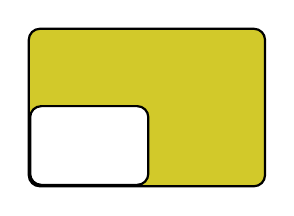
\begin{tikzpicture}[even odd rule, rounded corners, x=1.5cm, y=1cm]
  \filldraw[fill=yellow!80!black, thick, rounded corners] (0, 0) rectangle (2, 2) [xshift=0.5, yshift=0.5] (0, 0) rectangle (1, 1);
\end{tikzpicture}
  
\tikz{\filldraw[even odd rule, fill=yellow!80!black, thick, rounded corners] (0, 0) rectangle (2, 2) [xshift=0.5, yshift=0.5] (0, 0) rectangle (1, 1)}

% foreach
\foreach \x in {1, 2, 3} {$x = \x, $}
\tikz{\foreach \x in {-1, -0.5, ..., 1} {\draw (\x, 0) -- (\x, 1);}}

% nodes
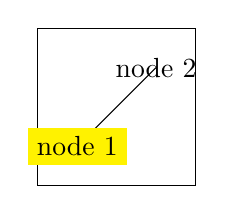
\begin{tikzpicture}
  \draw (0, 0) rectangle (2, 2);
  \draw (0.5, 0.5) node [fill=yellow] {node 1} -- (1.5, 1.5) node {node 2};
\end{tikzpicture}



% nodes
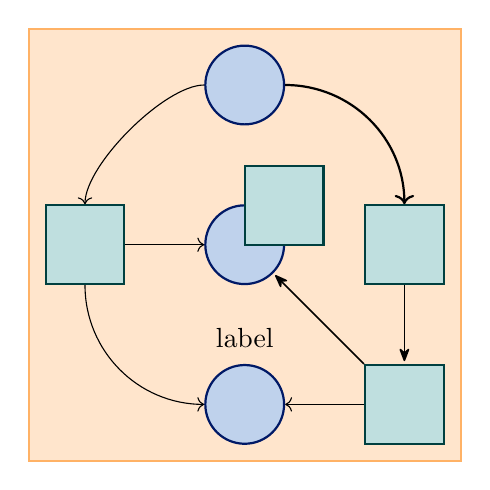
\begin{tikzpicture}[inner sep=2mm]
  % nodes
  \node at (0, 0) [circStyle] (middle){};
  \node [rectStyle] (left) [left=of middle]{};
  \node [rectStyle] (right) [right=of middle]{};
  \node [circStyle] (up) [above=of middle]{};
  \node [circStyle] (down) [below=of middle, label=above:label]{};
  \node at (0.5, 0.5) [rectStyle] (overlapp){};

  % lines
  \draw [->] (left.east) -- (middle.west);
  \draw [->] (up.west) .. controls +(left:5mm) and +(up:5mm) .. (left.north);
  \draw [->, thick] (up.east) to [out=0, in=90] (right.north);
  \draw [->] (left.south) to [bend right=45] (down.west);

  % edges
  \node [rectStyle] (karl) [below=of right]{} edge [->] (down) edge [pre] (right) edge [post] (middle);

  % background
  \begin{scope}[on background layer]
    \node [rectangle, draw=orange!60, thick, fill=orange!20, fit=(left) (right) (up) (down)] {};
  \end{scope}
\end{tikzpicture}

% frame test
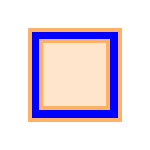
\begin{tikzpicture}
  \node [rectangle, draw=orange!60, thick, fill=orange!20, line width=2mm, minimum size=10mm] [postaction={draw, line width=1mm, blue}] {};
\end{tikzpicture}

% frame macro / style
\tikzset{pictureframepic/.pic={\node [draw=white, line width=2mm, fill=white, inner sep=0mm, postaction={draw, line width=1mm, orange!60}]{};}}
\tikzset{pictureframe/.style={draw=white, line width=2mm, fill=white, inner sep=0mm, postaction={draw, line width=1mm, orange!60}}}



% shading
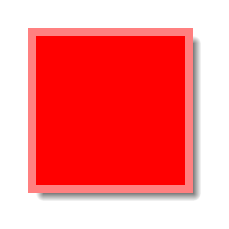
\begin{tikzpicture}

  % foreground image
  \node at (0, 0) (target) [draw=red!50, line width=1mm, fill=red, rectangle, minimum size=2cm] {};

  % background shading
  \begin{scope}[on background layer]

    % common coordinates
    \coordinate (A) at ([xshift=2mm] target.south west);
    \coordinate (B) at ($ (target.north east) + (0, -2mm) $);

    % ball shade
    \shade [shading=radial] (target.south east) circle (1mm);
    \shade [shading=radial] (A) circle (1mm);
    \shade [shading=radial] (B) circle (1mm);

    % rect shade
    \shade (A) rectangle ([yshift=-1mm] target.south east);
    \shade [shading angle=90] (B) rectangle ([xshift=1mm] target.south east);
  \end{scope}

\end{tikzpicture}


% fading
\tikzfading[name=fade out, inner color=transparent!0, outer color=transparent!100]


\tikzset{
  %%%% 
  % frame shading code
  %%%%
  %frameshade/.pic={
  pics/frameshade/.style args={#1/#2}{
    code = {
      % common coordinates
      \coordinate (A) at ([xshift=#2] #1.south west);
      \coordinate (B) at ([yshift=-#2] #1.north east);
      \coordinate (C) at (#1.south east);

      \begin{scope} \clip (#1.south west) rectangle ++(#2, -#2); \fill [color=black, path fading=fade out] (A) circle (#2); \end{scope}
      \begin{scope} \clip (#1.north east) rectangle ++(#2, -#2); \fill [color=black, path fading=fade out] (B) circle (#2); \end{scope}
      \begin{scope} \clip (C) rectangle ++(#2, -#2); \fill [color=black, path fading=fade out] (C) circle (#2); \end{scope}

      % shadow droping
      \fill [color=black, path fading=south] (A) rectangle ([yshift=-#2] #1.south east);
      \fill [color=black, path fading=east] (B) rectangle ([xshift=#2] #1.south east);
    }
  }
}


% blur shadow
\tikzset{my frame shade/.style={blur shadow={shadow opacity=90, shadow blur steps=5, shadow blur extra rounding=1pt, shadow xshift=2mm, shadow yshift=-2mm, shadow scale=1.0}, shadow blur radius=1mm, shadow blur steps=10}}

\begin{tikzpicture}
    
  % pattern
  \node at (0, 0) [rectangle, minimum size=3cm, pattern=checkerboard, pattern color=red] {};
  \node at (0, 0) (target) [draw=blue!50, line width=1mm, fill=blue, rectangle, minimum size=2cm] {};
  \pic {frameshade=target/5mm};

  % pattern
  \node at (3, 0) [rectangle, minimum size=3cm, pattern=checkerboard, pattern color=red] {};
  \node at (3, 0) (target) [draw=blue!50, line width=0.5mm, fill=blue, rectangle, minimum size=2cm, drop shadow={shadow scale=1.1}] {};

  % pattern
  \node at (6, 0) [rectangle, minimum size=3cm, pattern=checkerboard, pattern color=red] {};
  \node at (6, 0) (target) [draw=blue!50, line width=0.5mm, fill=blue, rectangle, minimum size=2cm, my frame shade] {};


\end{tikzpicture}


% positioning

\begin{tikzpicture}
  \fill (0, 0) circle (2mm);
  \fill [color=red] (0, 0) rectangle ++(2mm, 2mm);
  \fill [color=blue] (2mm, 0) rectangle ++(2mm, 2mm);
  \fill [color=red] (4mm, 0) rectangle ++(2mm, 2mm);

  \fill [color=red, path fading=south, fading transform={rotate=45}] (1, 0) rectangle ++(2mm, 2mm);
\end{tikzpicture}


% transparency

\begin{tikzpicture}[opacity=0.5]
  \draw [line width=5mm] (0, 0) -- (2, 2);
  \draw [line width=5mm] (2, 0) -- (0, 2);

  \begin{scope}[transparency group]
    \draw [line width=5mm] (3, 0) -- (5, 2);
    \draw [line width=5mm] (5, 0) -- (3, 2);
  \end{scope}
\end{tikzpicture}

% transparency

\begin{tikzpicture}
  \draw [line width=5mm, path fading=east] (0, 0) -- (2, 2);
  \draw [line width=5mm, path fading=east] (2, 0) -- (0, 2);

  \begin{scope}[transparency group]
    \pgfsetblendmode{exclusion}
    \draw [line width=5mm, path fading=east, red] (3, 0) -- (5, 2);
    \draw [line width=5mm, path fading=east, blue] (5, 0) -- (3, 2);
  \end{scope}
\end{tikzpicture}


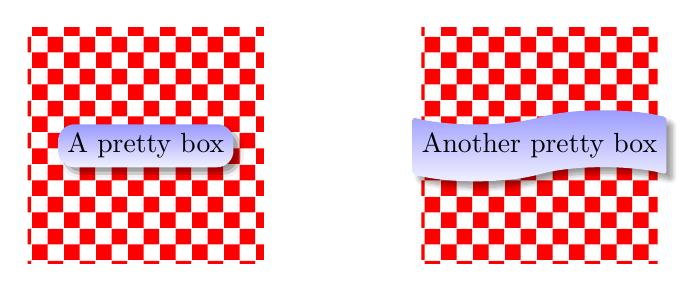
\begin{tikzpicture}

  % pattern
  \node at (0, 0) [rectangle, minimum size=3cm, pattern=checkerboard, pattern color=red] {};
  \node[draw=none, shade, top color=blue!40, bottom color=blue!5, rounded corners=6pt, blur shadow={shadow blur steps=2}] {A pretty box};

  % pattern
  \node at (5, 0) [rectangle, minimum size=3cm, pattern=checkerboard, pattern color=red] {};
  \node[tape, draw=none,shade, top color=blue!40, bottom color=blue!5, rounded corners=1pt, blur shadow={shadow blur steps=10, shadow blur extra rounding=1.3pt}] at (5,0){Another pretty box};

\end{tikzpicture}


\begin{tikzpicture}
  %%%
  % positioning
  %%%

  % pattern
  \node at (0, 0) (pattern) [rectangle, minimum size=3cm, pattern=checkerboard, pattern color=red] {};
  \fill [blue] (0, 0) rectangle ++(10pt, 10pt);
  \fill [blue!50] (pattern.south) rectangle ++(10pt, 20pt);
  \fill [blue!50] (pattern.north) rectangle ++(-10pt, 20pt);
  \fill [blue!50] (pattern.west) rectangle ++(10pt, 20pt);
  \fill [blue!50] (pattern.east) rectangle ++(10pt, -20pt);

  % pattern
  \node at (5, 0) (pattern) [rectangle, minimum size=3cm, pattern=checkerboard, pattern color=red] {};
  \node at (pattern.north) [rectangle, fill=blue!30, inner sep=10pt, anchor=north] {};
  \node at (pattern.south) [rectangle, fill=blue!30, inner sep=10pt] {};
  \node at (pattern.west) [rectangle, draw, line width=5pt, fill=blue!30, inner sep=10pt, anchor=west, my frame shade] {};
  \node at (pattern.west) [rectangle, fill=blue!30, inner sep=10pt, anchor=west, yshift=1cm] {};
  \node at (pattern.east) [rectangle, draw, line width=5pt, fill=blue!30, inner sep=10pt, anchor=east, my frame shade] {};
\end{tikzpicture}


\newpage
\begin{tikzpicture}[remember picture, overlay]
  %%%
  % overlays
  %%%
  \fill (current page.center) circle (10pt) node [above] {center};
  \fill (current page.south) circle (10pt) node [above] {south};
  \fill (current page.south west) circle (10pt) node [above] {south west};
\end{tikzpicture}


% animations?
% \tikz \node [animate = { myself: = { begin on = click, scope = { attribute = fill, repeats = 3, 0s = "red", 2s = "red!50" }, scope = { attribute = draw, 0s = "red", 2s = "red!50" } }}, fill=blue!20, draw=blue, very thick, circle] {Click me};

% \begin{tikzpicture}[ animate/orbit/.style 2 args = { myself:shift = { along = { (0,0) circle [radius=#1] } sloped in #2s/10, repeats }} ] \node :color = {0s = "orange", 2s = "red", 4s = "orange", repeats} {Sun}; \begin{scope}[animate={orbit={2.5cm}{365}}] \node {Earth}; \node [animate={orbit={1cm}{28}}] {Moon}; \end{scope} \useasboundingbox (-3.8,-3.8) (3.8,3.8); \end{tikzpicture}

\end{document}